
\chapter{Methods}

\section{Dataset}

This thesis uses the VocalSet dataset \cite{wilkins_vocalset:_2018}. The dataset consists of sung vowel excerpts from 20 singers (9 female, 11 male). For each singer, five vowels are sung in different arrangements (single notes, arpeggios and scales) and different singing techniques (vibrato, straight, breathy,...). 

\section{Singing Voice Synthesis}

\begin{figure}[H]
    \centering
    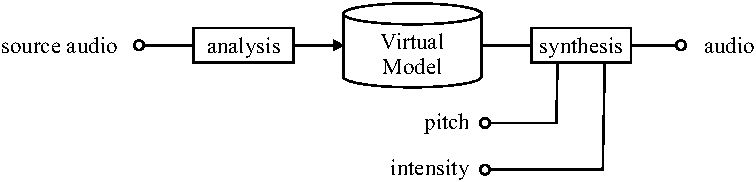
\includegraphics{Graphics/005_method_singer_model.pdf}
    \caption{A singer model is trained from source audio material. The model is used with pitch and control parameters to generate new sung vowels.}
    \label{fig:singer_model}
\end{figure}

In this thesis, we aim to propose a singing voice synthesis method for the synthesis of sung vowels. For this purpose, we train virtual singer model using target source samples from the VocalSet. During synthesis, these models can be used with control parameters pitch and intensity to synthesize new excerpts. Furthermore, singer models can be morphed, either during analysis or synthesis, to blend between voice timbre qualities. An overview is shown in figure \ref{fig:singer_model}.\\

After reviewing the current sate of research, three types of approaches were deemed suitable. These include end-to-end \textbf{audio prediction} approaches like WaveNet \cite{oord_wavenet:_2016}, spectral envelope / \textbf{vocoder prediction} approaches like WGANSing \cite{chandna_wgansing:_2019} and \textbf{extended source-filter} models extracted from source audio \cite{schleusing_joint_2013}. These three  approaches differ in abstraction, required domain knowledge and computational efficiency. Audio prediction methods achieve very good results with low required domain knowledge at the cost of accuracy while extended source filter models require a high level of domain knowledge and perform worse then state at the art methods for the benefit of computational efficiency. A comparison is shown in figure \ref{fig:method_comparison}. In the following sections, all three approaches are briefly introduced. 

\begin{figure}[H]
    \centering
    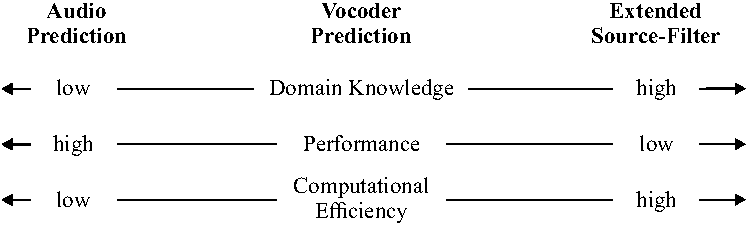
\includegraphics{Graphics/006_method_compairson.pdf}
    \caption{Compared to extended source-filter models, audio predictor approaches trade low required domain knowledge and a better accuracy with a low computational efficiency.}
    \label{fig:method_comparison}
\end{figure}

\subsection*{End-to-End Audio Predictor Methods}

\begin{figure}[H]
    \centering
    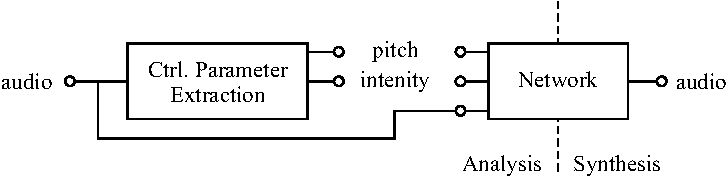
\includegraphics{Graphics/007_method_audio_predictor.pdf}
    \caption{Exemplary architecture of analysis and synthesis of audio predictor  singing voice synthesis methods.}
    \label{fig:method_audio_predictor}
\end{figure}

Audio predictor methods use deep neural networks to predict audio samples based on past predicted audio samples and conditioning signals such as pitch and intensity \cite{oord_wavenet:_2016}. One possible architecture is shown in figure \ref{fig:method_audio_predictor}. During analysis, pitch and intensity trajectories have to be extracted from the source samples. The network is trained to predict new samples in the source audio by observing past samples and the conditioning signals. During synthesis, the network is used to predict new samples based on previously predicted samples (autorregression) and controlled via conditioning signals. A multi singer model can be trained by using multiple singer source samples together with a singer ID one-hot vector as conditioning signal during training. \\
End-to-End audio predictors are usually very complex due to the complexity of the task that the networks are responsible of \cite{engel_ddsp:_2020}.

\subsection*{Vocoder Predictor Methods}

\begin{figure}[H]
    \centering
    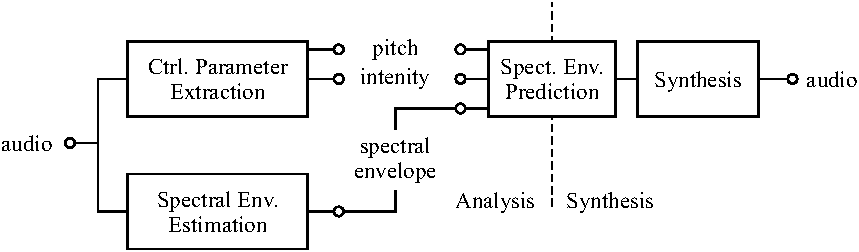
\includegraphics{Graphics/008_method_vocoder_predictor.pdf}
    \caption{Exemplary architecture of analysis and synthesis of vocoder predictor singing voice synthesis methods. }
    \label{fig:method_vocoder}
\end{figure}

Vocoder predictor methods are based on the source-filter model. One possible architecture is shown in figure \ref{fig:method_vocoder}. Instead or predicting raw audio, they predict coefficients for a spectral envelope that can be used together with pitch and additional parameters to synthesize the audio. In  \cite{blaauw_neural_2017-1}, WaveNet was used to the predict the envelope coefficients autorregressively. Various vocoders can be used to extract spectral envelopes and synthesis audio \cite{morise_world:_2016}. One possible advantage over audio predictors is the reduced complexity of predicting spectral envelope parameters \cite{engel_ddsp:_2020}. Having access to spectral envelopes prior to synthesis also allows us to morph between singer models by interpolating between spectral envelopes prior to synthesis, for instance using their LSF representation \cite{roddy_method_2014}. 

\section*{Extended Source-Filter}
    
\begin{figure}[H]
    \centering
    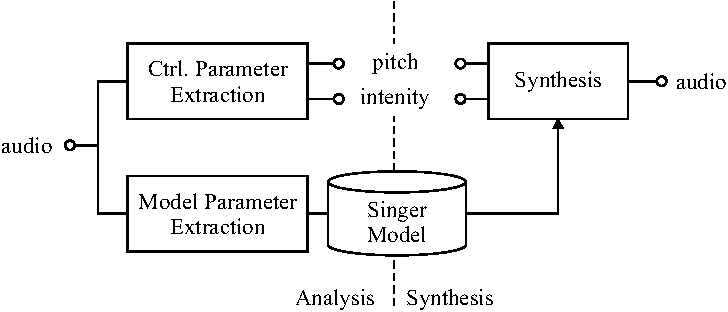
\includegraphics{Graphics/009_method_extended_source_filter.pdf}
    \caption{Exemplary architecture of analysis and synthesis of an extended source filter model for singing voice synthesis methods. }
    \label{fig:method_esf}
\end{figure}

Extended source-filter models require a high level of domain knowledge. The model would not only need to model vocal tract and glottal flow but also would need to model the dependency between control parameters pitch and intensity and the synthesis parameters for vocal tract and spectral envelope. During analysis, all parameters need to be estimated from the source sample. During synthesis, most parts of the model could be implemented using classical signal processing. This dramatically reduces the computational cost compared to the previously presented methods.\\
With vocal tract and glottal flow separated, morphing can be accomplished by interpolating their parameters respectively, again using representations such as LSF to achieve good results.

\subsection*{Differentiable DSP}

DDSP \cite{engel_ddsp:_2020} seems very promising but can't be easily applied to this thesis problem. As mentioned earlier, DDSP combines machine learning with classical DSP but requires the used DSP components to be differentiable. The commonly used model of the vocal tract as an all pole system however is not differentiable. With this limitation, no clean vocal tract separation could be achieved and DDSP could instead only be used to predict coefficients for a sinusoidal plus noise model \cite{serra_musical_1997}.

\subsection*{Summary - Singing Voice Synthesis Methods}

All three presented methods are suitable for implementing singing voice synthesis. However, with the computational complexity of audio prediction and vocoder prediction, an extended source-filter model is the currently preferred method considering the requirements mentioned earlier.\\

\section{Evaluation}

Evaluation of the proposed method is supposed to answer the following questions. Is the proposed method capable of recreating sung vowel excerpts to a satisfactory level? Can the method be used to synthesize sung vowel excerpts perceived as realistic or natural by listeners? Does the proposed model fulfil the strict real time requirements imposed on it? To answer the first two questions, an empirical user test is proposed. Since no hardware is necessary for this test, we suggest conducting an online survey to increase the potential number of participants. 

For measuring the perceived difference between original and synthesized excerpts, a MUSHRA (MUltiple Stimuli with Hidden Reference and Anchor) \cite{itu-r_recommendation_bs.1534_method_2003} test is proposed \cite{morise_cheaptrick_2015}\cite{morise_world:_2016}\cite{blaauw_neural_2017-1}. Alternatively, for small audibly differences, ABC-HR (ABC-Hidden Reference) \cite{itu-r_recommendation_bs.1534_method_2003} can be used instead. The synthesized excerpt is generated using the control parameter trajectories extracted from the original excerpt so that  the synthesized excerpt ideally is perceptually identical to the original excerpt. 

Additionally, some aspects of the method can be evaluated by performing a subjective paired comparison test as proposed in \cite{oord_wavenet:_2016}. In this test, the participants are asked to listen to two samples and state which they prefer with the option to choose "neutral". In all tests, sample $A$ is synthesized directly from model $A$ using the control parameters extracted from the original source audio sample $A$. If the method performs well, we expect a neutral response regarding which sample the participants prefer.

\begin{itemize}
    \item \textbf{Separation of voice timbre qualities and expressive qualities.}\\
    Sample $A$ is compared with an audio sample generated by using the same model $A$ but control parameters extracted from original sample $B$. This test measures how well a model transitions from it's original set of control parameters to a new set of control parameters.  
    \item \textbf{Voice Morphing Capabilities}\\
    The synthesized sample $A$ is compared with the synthesized sample $A \times B$, created by morphing models $A$ and $B$, using the same control parameters as with sample $A$. This test measures how well a morph between models maintains the naturalness of the voice.
\end{itemize}